% -*- latex -*-
%%%%%%%%%%%%%%%%%%%%%%%%%%%%%%%%%%%%%%%%%%%%%%%%%%%%%%%%%%%%%%%%
%%%%%%%%%%%%%%%%%%%%%%%%%%%%%%%%%%%%%%%%%%%%%%%%%%%%%%%%%%%%%%%%
%%%%
%%%% This text file is part of the lecture slides for
%%%% `Parallel Computing'
%%%% by Victor Eijkhout, copyright 2012-2020
%%%%
%%%% Collective-slides.tex : slides about collective operations
%%%%
%%%%%%%%%%%%%%%%%%%%%%%%%%%%%%%%%%%%%%%%%%%%%%%%%%%%%%%%%%%%%%%%
%%%%%%%%%%%%%%%%%%%%%%%%%%%%%%%%%%%%%%%%%%%%%%%%%%%%%%%%%%%%%%%%

\begin{frame}[containsverbatim]{Overview}
  In this section you will learn `collective' operations, that combine
  information from all processes.

  Commands learned:
  \begin{itemize}
  \item \indexmpishow{MPI_Bcast}, \indexmpishow{MPI_Reduce}, \indexmpishow{MPI_Gather}, \indexmpishow{MPI_Scatter}
  \item \indexmpishow{MPI_All_...} variants, \indexmpishow{MPI_....v} variants
  \item \indexmpishow{MPI_Barrier}, \indexmpishow{MPI_Alltoall}, \indexmpishow{MPI_Scan}
  \end{itemize}
\end{frame}

\begin{frame}{Technically}
  Routines can be `collective on a communicator': 
  \begin{itemize}
  \item They involve a communicator;
  \item if one process calls that routine, every process in that
    communicator needs to call it
  \item Mostly about combining data, but also opening shared files,
    declaring `windows' for one-sided communication.
  \end{itemize}
\end{frame}

\sectionframe{Concepts}

\begin{frame}[containsverbatim]\frametitle{Collectives}
  Gathering and spreading information:
  \begin{itemize}
  \item Every process has data, you want to bring it together;
  \item One process has data, you want to spread it around.
  \end{itemize}
  Root process: the one doing the collecting or disseminating.

  Basic cases:
  \begin{itemize}
  \item Collect data: gather.
  \item Collect data and compute some overall value (sum, max): reduction.
  \item Send the same data to everyone: broadcast.
  \item Send individual data to each process: scatter.
  \end{itemize}
\end{frame}

\frame{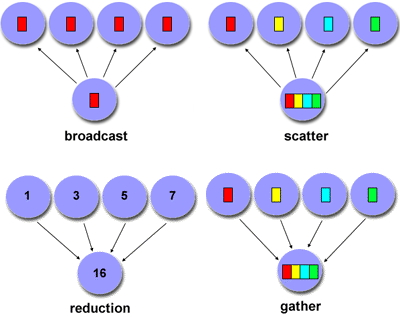
\includegraphics[scale=.8]{collective_comm}}

\begin{exerciseframe}
  \input ex:collective-cases
\end{exerciseframe}

\begin{frame}[containsverbatim]\frametitle{More collectives}
  \begin{itemize}
  \item Instead of a root, collect to all: \indexmpishow{MPI_All...}
  \item Scatter/Gather individual data, but also individual size:
    \indexmpishow{MPI_Scatterv}, \indexmpishow{MPI_Allgatherv} et cetera.
  \item Everyone broadcasts: \indexmpishow{MPI_Alltoall}
  \item Scan: like a reduction, but with partial results
  \item Non-blocking collectives.
  \end{itemize}
\end{frame}

\sectionframe{Basic collectives}

\begin{frame}{Motivation for allreduce}
Standard deviation:
\[ \sigma = \sqrt{\frac1N \sum_i^N (x_i-\mu) }
\qquad\hbox{where}\qquad \mu = \frac{\sum_i^Nx_i}N
\]
and assume that every processor stores just one~$x_i$ value.

How do we compute this?
\begin{enumerate}
\item<2-> The calculation of the average~$\mu$ is a reduction.
\item<3-> Every
  process needs to compute~$x_i-\mu$ for its value~$x_i$, so use
  allreduce operation, which does the reduction and leaves
  the result on all processors.
\item<4-> $\sum_i(x_i-\mu)$ is another sum of
  distributed data, so we need another reduction operation. Might as
  well use alreduce.
\end{enumerate}
\end{frame}

\begin{frame}[containsverbatim]{Another Allreduce}
  Example: normalizing a vector
  \[ y \leftarrow x/\|x\| \]
  \begin{itemize}
  \item Vectors \n{x,y} are distributed: every process has certain
    elements
  \item The norm calculation is an all-reduce: every process gets same
    value
  \item Every process scales its part of the vector.
  \end{itemize}
\end{frame}

\begin{frame}{Reduction to single process}
    Regular reduce: great for printing out summary information at the
  end of your job.
\end{frame}

\begin{frame}[containsverbatim]{Allreduce syntax}
\begin{lstlisting}
  int MPI_Allreduce(
    const void* sendbuf,
    void* recvbuf, int count, MPI_Datatype datatype,
    MPI_Op op, MPI_Comm comm)  
\end{lstlisting}
\begin{itemize}
\item All processes have send and recv buffer
\item (No root argument)
\item \n{count} is number of items in the buffer: 1~for scalar.
\item \indexmpishow{MPI_Datatype} is \indexmpishow{MPI_INT}, \indexmpishow{MPI_REAL8} et cetera.
\item \indexmpishow{MPI_Op} is \indexmpishow{MPI_SUM}, \indexmpishow{MPI_MAX} et cetera.
\end{itemize}
\end{frame}

\begin{frame}[containsverbatim]{Elementary datatypes}
\begin{tabular}{|l|l|l|}
  \hline
  C&Fortran&meaning\\
  \hline
  \indexmpishow{MPI_CHAR}&  \indexmpishow{MPI_CHARACTER}&only for text\\
  \indexmpishow{MPI_SHORT}&  \indexmpishow{MPI_BYTE}&8 bits\\
  \indexmpishow{MPI_INT}&  \indexmpishow{MPI_INTEGER}&like the C/F types\\
  \indexmpishow{MPI_FLOAT}&  \indexmpishow{MPI_REAL}&\\
  \indexmpishow{MPI_DOUBLE}&  \indexmpishow{MPI_DOUBLE_PRECISION}&\\
  &\indexmpishow{MPI_COMPLEX}&\\
  &\indexmpishow{MPI_LOGICAL}&\\  
  \hline
  &&internal use\\
  \hline
  &&\indexmpishow{MPI_Aint}\\
  &&\indexmpishow{MPI_Offset}\\
  \hline
\end{tabular}  

A bunch more.
\end{frame}

\begin{frame}[containsverbatim]{MPI operators}
\begingroup \tt\catcode`\_=12\relax %pyskip
\begin{tabular}{|l|l|}
  \hline
  \indexmpishow{MPI operator}&description\\
  \hline
  \indexmpishow{MPI_MAX}&maximum\\
  \indexmpishow{MPI_MIN}&minimum\\
  \indexmpishow{MPI_SUM}&sum\\
  \indexmpishow{MPI_PROD}&product\\
  \indexmpishow{MPI_LAND}&logical and\\
  \indexmpishow{MPI_BAND}&bitwise and\\
  \indexmpishow{MPI_LOR}&logical or\\
  \indexmpishow{MPI_BOR}&bitwise or\\
  \indexmpishow{MPI_LXOR}&logical xor\\
  \indexmpishow{MPI_BXOR}&bitwise xor\\
  \hline
\end{tabular}
\endgroup %pyskip

A couple more.
\end{frame}

\begin{frame}[containsverbatim]\frametitle{Buffers in C}
  General principle: buffer argument is address in memory of the data.
  \begin{itemize}
  \item Buffer is void pointer: 
  \item write \n{&x} or \n{(void*)&x} for scalar
  \item write \n{x} or \n{(void*)x} for array
  \end{itemize}
\end{frame}

\begin{frame}[containsverbatim]\frametitle{Buffers in Fortran}
  General principle: buffer argument is address in memory of the data.
  \begin{itemize}
  \item Fortran always passes by reference:
  \item write \n{x} for scalar
  \item write \n{x} for array
  \end{itemize}
\end{frame}

\begin{frame}[containsverbatim]\frametitle{Buffers in Python}
  For many routines there are two variants:
  \begin{itemize}
  \item lowercase: can send Python objects;\\
    output is \n{return} result\\
\begin{verbatim}
result = comm.recv(...)
\end{verbatim}
    this uses \n{pickle}: slow.
  \item uppercase: communicates \n{numpy} objects;\\
    input and output are function argument.
\begin{verbatim}
result = np.empty(.....)
comm.Recv(result, ...)
\end{verbatim}
    basicaly wrapper around C code: fast
  \end{itemize}
\end{frame}

\begin{exerciseframe}[randommax]
  \input ex:randommaxscale
\end{exerciseframe}

\begin{frame}[containsverbatim]{Random numbers in C}
\lstset{language=C}
\begin{lstlisting}
// Initialize the random number generator
srand(procno*(double)RAND_MAX/nprocs);
// compute a random number
randomfraction = (rand() / (double)RAND_MAX);
\end{lstlisting}
\end{frame}

\begin{frame}[containsverbatim]{Random numbers in Fortran}
\lstset{language=Fortran}
\begin{lstlisting}
integer :: randsize
integer,allocatable,dimension(:) :: randseed
real :: random_value

call random_seed(size=randsize)
allocate(randseed(randsize))
randseed(:) = 1023*procno
call random_seed(put=randseed)

call random_number(random_value)
\end{lstlisting}
\end{frame}

\begin{frame}[containsverbatim]{Random numbers in Python}
\lstset{language=Python}
\begin{lstlisting}
import random

random.seed(procno)

random_value = random.random()
\end{lstlisting}
\end{frame}

\begin{optexerciseframe}
  \input ex:randomcoord
\end{optexerciseframe}

\begin{frame}[label=reduce,containsverbatim]{Reduction to root}
\lstset{language=C}
\begin{lstlisting}
int MPI_Reduce
  (void *sendbuf, void *recvbuf,
   int count, MPI_Datatype datatype, 
   MPI_Op op, int root, MPI_Comm comm)
\end{lstlisting}
\begin{itemize}
\item Buffers: \n{sendbuf}, \n{recvbuf} are ordinary variables/arrays.
\item Every process has data in its \n{sendbuf},\\
  Root combines it in \n{recvbuf} (ignored on non-root processes).
\item \n{count} is number of items in the buffer: 1~for scalar.
\item \indexmpishow{MPI_Op} is \indexmpishow{MPI_SUM}, \indexmpishow{MPI_MAX} et cetera.
\end{itemize}
\end{frame}

%% \begin{longcourse}
%%   \begin{exerciseframe}
%%     \input ex:argv-bcast
%%   \end{exerciseframe}
%% \end{longcourse}

%% \begin{full}
%%   \begin{exerciseframe}[randommax]
%%     \input ex:randommax
%%   \end{exerciseframe}
%% \end{full}

\begin{frame}[label=bcast,containsverbatim]\frametitle{Broadcast}
\begin{lstlisting}
int MPI_Bcast(
    void *buffer, int count, MPI_Datatype datatype, 
    int root, MPI_Comm comm )
\end{lstlisting}
\begin{itemize}
\item All processes call with the same argument list
\item \n{root} is the rank of the process doing the broadcast
\item Each process allocates buffer space;\\
  root explicitly fills in values,\\
  all others receive values through broadcast call.
\item Datatype is \indexmpishow{MPI_FLOAT}, \indexmpishow{MPI_INT} et cetera, different
  between C/Fortran.
\item \n{comm} is usually \indexmpishow{MPI_COMM_WORLD}
\end{itemize}
\end{frame}

\begin{frame}{Allreduce vs Reduce/Bcast}
  Allreduce is equivalent to reduce and broadcast.
  \begin{itemize}
  \item One line less code.
  \item Gives the implementation more possibilities for optimization.
  \item Is actually twice as fast: allreduce same time as reduce.
  \end{itemize}
\end{frame}

\begin{frame}{Gauss-Jordan elimination}
  \url{https://youtu.be/aQYuwatlWME}
\end{frame}

\begin{exerciseframe}[jordan]
  \small
  \input ex:gaussjordancoll
\end{exerciseframe}

\begin{optexerciseframe}
  Bonus exercise: can you extend your program to have multiple columns
  per processor?
\end{optexerciseframe}

\sectionframe{Gather/Scatter, Scan, Barrier, and others}

\begin{frame}[containsverbatim]\frametitle{Gather/Scatter}
{\small
\begin{lstlisting}
int MPI_Gather(
  void *sendbuf, int sendcnt, MPI_Datatype sendtype,
  void *recvbuf, int recvcnt, MPI_Datatype recvtype,
  int root, MPI_Comm comm
);
int MPI_Scatter
  (void* sendbuf, int sendcount, MPI_Datatype sendtype, 
   void* recvbuf, int recvcount, MPI_Datatype recvtype, 
   int root, MPI_Comm comm) 
\end{lstlisting}
}
\begin{itemize}
\item Compare buffers to \hyperlink{reduce}{\beamergotobutton{reduce}}
\item Scatter: the \n{sendcount} / Gather: the \n{recvcount}:\\
this is not, as you might expect, the total length of the
buffer; instead, it is the amount of data to/from each process.
\end{itemize}
\end{frame}

\begin{frame}{Gather pictured}
  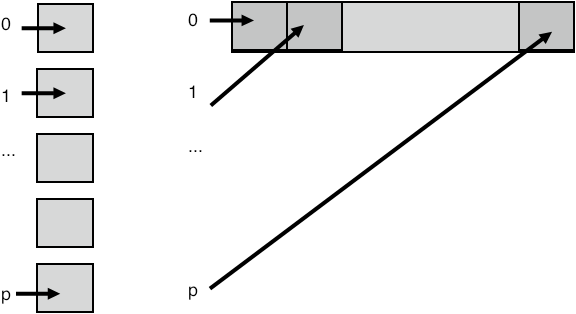
\includegraphics[scale=.4]{gather}
\end{frame}

\begin{exerciseframe}
  \input ex:randomwhere
\end{exerciseframe}

\begin{frame}{Popular application of gather}
  Matrix is constructed distributed, but needs to be brough to one
  process:
  
  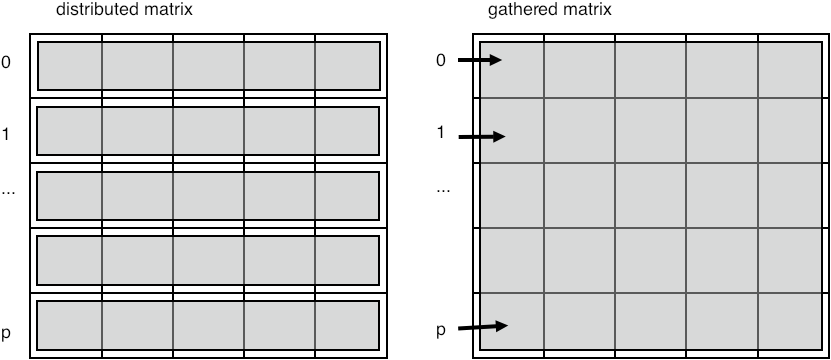
\includegraphics[scale=.4]{allgathermatrix}

  This is not efficient in time or space. Do this
  only when strictly necessary. Remember SPMD: try to keep everything
  symmetrically parallel. 
\end{frame}

\protoslide{MPI_Allgather}

\begin{frame}{Allgather pictured}
  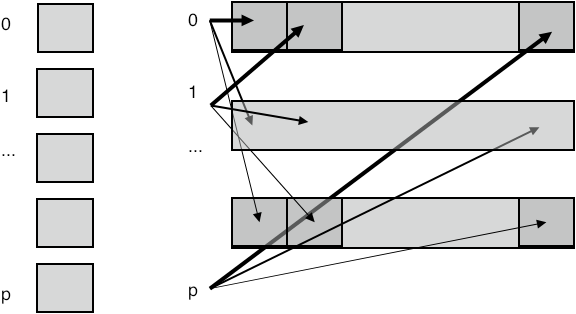
\includegraphics[scale=.4]{allgather}
\end{frame}

\begin{frame}[containsverbatim]\frametitle{Scan}
Scan or `parallel prefix': reduction with partial results

\begin{itemize}
\item Useful for indexing operations:
\item Each process has an array of $n_p$ elements;
\item My first element has global number $\sum_{q<p}n_q$.
\item Two variants: \indexmpishow{MPI_Scan} inclusive, and
  \indexmpishow{MPI_Exscan} exclusive.
\end{itemize}
\end{frame}

\begin{longcourse}
  \protoslide{MPI_Scan}
\end{longcourse}

\begin{frame}[containsverbatim]\frametitle{V-type collectives}
  \begin{itemize}
  \item Gather/scatter but with individual sizes
  \item Requires displacement in the gather/scatter buffer
  \end{itemize}
\end{frame}

\protoslide{MPI_Gatherv}

\begin{frame}[containsverbatim]\frametitle{All-to-all}
  \begin{itemize}
  \item Every process does a scatter;
  \item (equivalently: every process gather)
  \item each individual data, but amounts are identical
  \item Example: data transposition in FFT
  \end{itemize}
\end{frame}

\begin{frame}{Data transposition}
  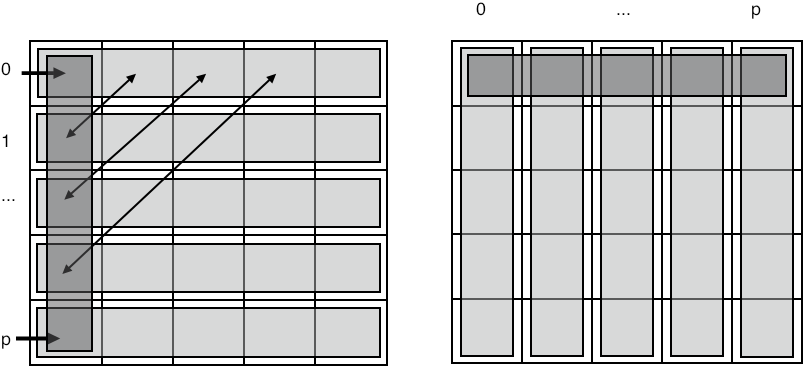
\includegraphics[scale=.4]{alltoall}

  Example: each process knows who to send to, \\
  all-to-all gives information who to receive from
\end{frame}

\begin{frame}[containsverbatim]\frametitle{All-to-allv}
  \begin{itemize}
  \item Every process does a scatter or gather;
  \item each individual data and individual amounts.
  \item Example: radix sort by least-significant digit.
  \end{itemize}
\end{frame}

\begin{frame}{Radix sort}
  \scriptsize
  Sort 4 numbers on two processes:

  \begin{tabular}{|r|rr|rrr|}
    \hline
    & \multicolumn{2}{|c}{proc0}&\multicolumn{3}{|c|}{proc1}\\
    array     & 2&5&7&1&\\
    binary    & 010& 101& 111& 001&\\
    \hline
    \multicolumn{6}{|c|}{stage 1}\\
    \hline
    last digit&   0&   1&   1&   1&\\
    &\multicolumn{5}{|c|}{(this serves as bin number)}\\
    sorted    & 010&    & 101& 111& 001\\
    \multicolumn{6}{|c|}{stage 2}\\
    \hline
    next digit&  1 &    &  0 &  1 &  0\\
    &\multicolumn{5}{|c|}{(this serves as bin number)}\\
    sorted    & 101& 001& 010& 111&\\
    \multicolumn{6}{|c|}{stage 3}\\
    \hline
    next digit& 1  & 0  & 0  & 1&\\
    &\multicolumn{5}{|c|}{(this serves as bin number)}\\
    sorted    & 001& 010& 101& 111&\\
    decimal   & 1  & 2  & 5  & 7&\\
    \hline
  \end{tabular}
\end{frame}

\begin{frame}[containsverbatim]{Reduce-scatter}
  \begin{itemize}
  \item 
    Pointwise reduction (one element per process) followed by scatter
  \item 
    Somewhat related to all-to-all: data transpose but reduced
    information, rather than gathered.
  \item Applications in both sparse and dense matrix-vector product.
  \end{itemize}
\end{frame}

\begin{frame}{Example: sparse matrix setup}
  Example: each process knows who to send to, \\
  all-to-all gives information how many messages to expect\\
  reduce-scatter leaves only relevant information

  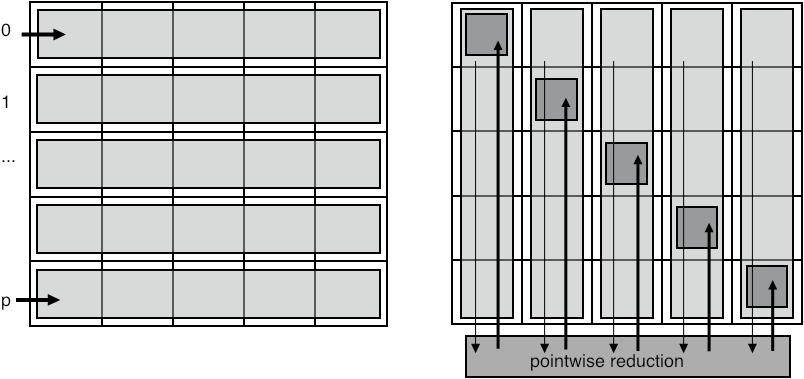
\includegraphics[scale=.4]{reducescatter}
\end{frame}

\begin{frame}[containsverbatim]\frametitle{Barrier}
\begin{lstlisting}
int MPI_Barrier( MPI_Comm comm )
\end{lstlisting}
  \begin{itemize}
  \item Synchronize processes:
  \item each process waits at the barrier until all processes have reached the barrier
  \item \textbf{This routine is almost never needed}:\\
    collectives are already a barrier of sorts, two-sided
    communication is a local synchronization
  \item One conceivable use: timing
  \end{itemize}
\end{frame}

\sectionframe{User-defined operators}

\begin{frame}[containsverbatim]\frametitle{MPI Operators}
  Define your own reduction operator
  \begin{itemize}
  \item Define operator between partial result and new operand
\lstset{language=C}
\begin{lstlisting}
typedef void MPI_User_function
    ( void *invec, void *inoutvec, int *len, 
      MPI_Datatype *datatype); 
\end{lstlisting}
\lstset{language=Fortran}
\begin{lstlisting}
FUNCTION user_function( invec(*), inoutvec(*), length, mpitype)
<fortrantype> :: invec(length), inoutvec(length) 
INTEGER :: length, mpitype
\end{lstlisting}
\item Don't forget to free:
\lstset{language=C}
\begin{lstlisting}
int MPI_Op_free(MPI_Op *op)  
\end{lstlisting}
\item Make your own reduction scheme \indexmpishow{MPI_Reduce_local}
  \end{itemize}
\end{frame}

\protoslide{MPI_Op_create}

\begin{frame}[containsverbatim]\frametitle{Example}
  Smallest nonzero:
  
  \cverbatimsnippet{mpirwz}
\end{frame}

\sectionframe{Performance of collectives}

\begin{frame}{Naive realization of collectives}
  Broadcast:
  
  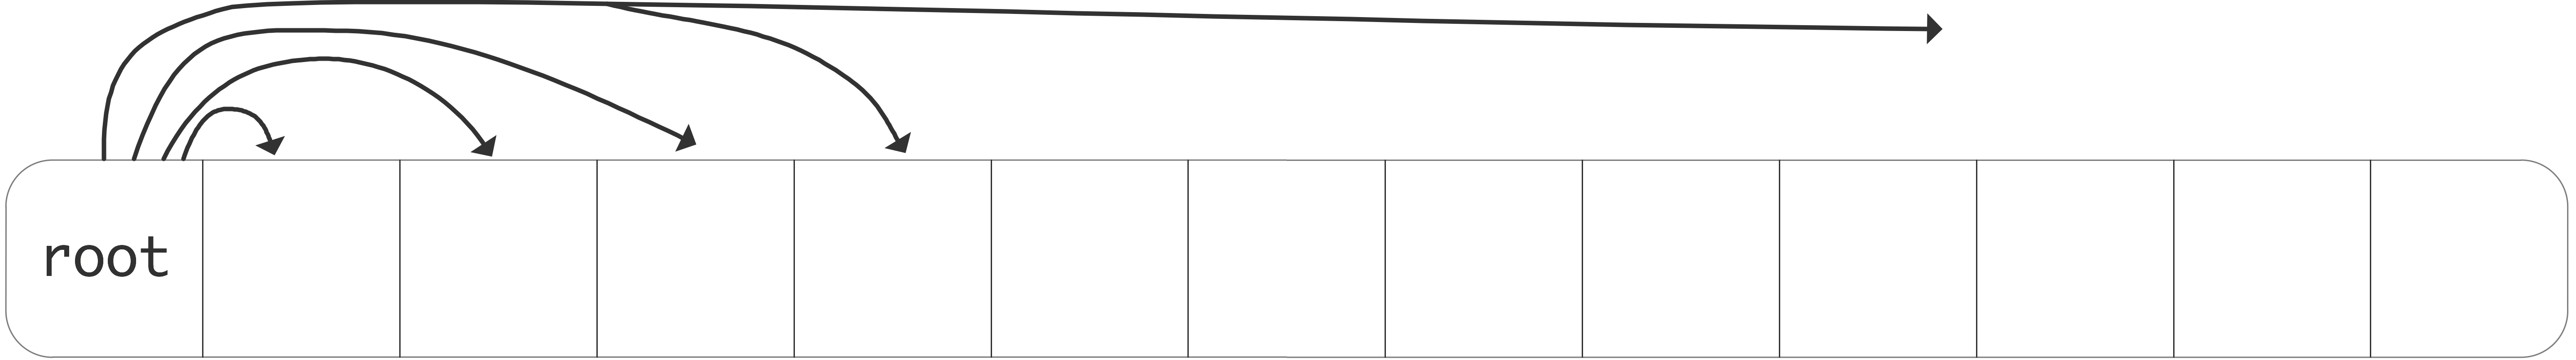
\includegraphics[scale=.06]{graphics/bcast-simple}

  Single message:
  \[ \alpha=\hbox{message startup}\approx 10^{-6}s,\qquad
  \beta=\hbox{time per word}\approx 10^{-9}s
  \]
  \begin{itemize}
  \item<2->Time for message of $n$ words: \[ \alpha +\beta n \]
  \item<3->Time for collective? Can you improve on that?
  \end{itemize}

\end{frame}

\begin{frame}{Better implementation of collective}
  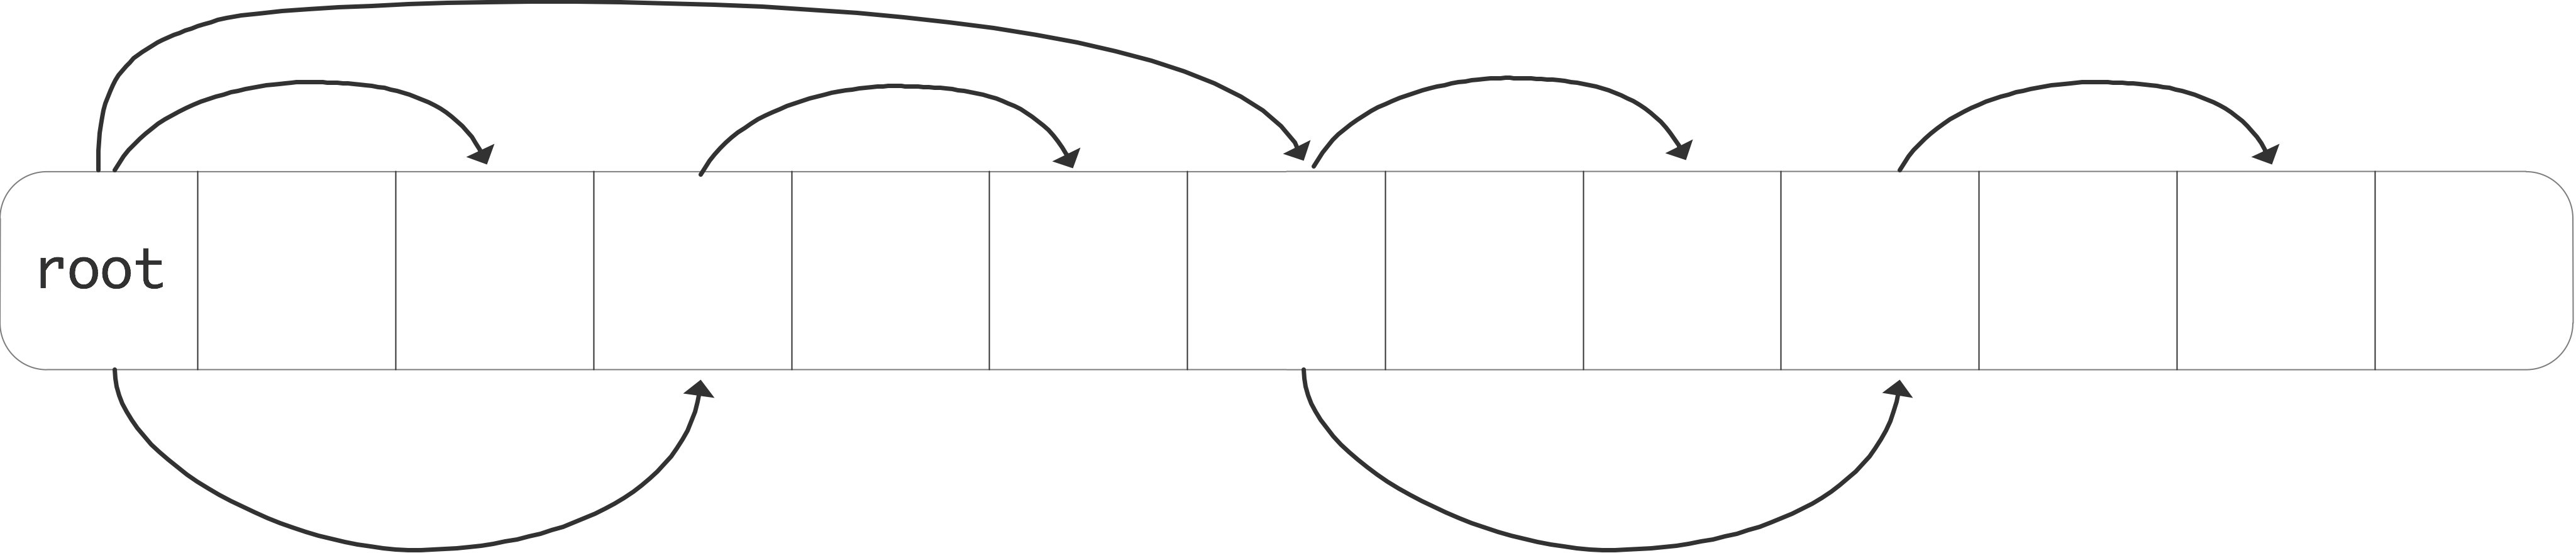
\includegraphics[scale=.07]{graphics/bcast-tree}
  
  \begin{itemize}
  \item<1->
    What is the running time now?
  \item<2->
    Can you come up with lower bounds on the $\alpha,\beta$ terms? Are
    these achieved here?
  \item<3-> How about the case of really long buffers?
  \end{itemize}

\end{frame}

\endinput

\begin{frame}[containsverbatim]\frametitle{}
\begin{lstlisting}
  
\end{lstlisting}
\end{frame}

\begin{frame}[containsverbatim]\frametitle{}
\begin{lstlisting}
  
\end{lstlisting}
\end{frame}

\begin{frame}[containsverbatim]\frametitle{}
\begin{verbatim}
  
\end{verbatim}
\end{frame}

